% ОБЯЗАТЕЛЬНО ИМЕННО ТАКОЙ documentclass!
% (Основной кегль = 14pt, поэтому необходим extsizes)
% Формат, разумеется, А4
% article потому что стандарт не подразумевает разделов
% Глава = section, Параграф = subsection
% (понятия "глава" и "параграф" из стандарта)
\documentclass[a4paper,article,14pt]{extarticle}

% Подключаем главный пакет со всем необходимым
\usepackage{spbudiploma_tempora}

% Пакеты по желанию (самые распространенные)
% Хитрые мат. символы
\usepackage{euscript}
% Таблицы
\usepackage{longtable}
\usepackage{makecell}
% Картинки (можно встявлять даже pdf)
\usepackage[pdftex]{graphicx}

\usepackage{amsthm,amssymb, amsmath}

% доп символы
\usepackage{textcomp}
\usepackage{dsfont}

% оформление алгоритма
\usepackage[ruled,vlined]{algorithm2e}

\begin{document}

% Титульник в файле titlepage.tex
% Титульный лист диплома СПбГУ
% Временное удаление foot на titlepage
\newgeometry{left=30mm, top=20mm, right=15mm, bottom=20mm, nohead, nofoot}
\begin{titlepage}
\begin{center}
% Первый символ съедается, первым знаком поставлен Ы
\textbf{Санкт--Петербургский}
\textbf{государственный университет}

\vspace{35mm}

\textbf{\textit{\large Тихонков Сергей Алексеевич}} \\[8mm]
% Название
\textbf{\large Выпускная квалификационная работа}\\[3mm]
\textbf{\textit{\large Исследование и применение алгоритмов на базе консенсуса для распределенного обучения нейронных сетей}}

\vspace{20mm}
% Булшит
Уровень образования: бакалавриат\\
Направление 02.03.02 «Фундаментальная информатика и информационные технологии»\\
Основная образовательная программа СВ.5003.2017
«Программирование и информационные технологии»\\
Профиль «Автоматизация научных исследований»\\[30mm]


% Научный руководитель, рецензент
% Сходить в уч отдел и узнать, правильно ли
\begin{flushright}
{Научный руководитель:} \\
профессор, кафедра математического моделирования энергетических систем, д.ф. - м.н.  Крылатов~Александр Юрьевич
\end{flushright}
\begin{flushright}
{Рецензент:} \\
доцент, зав. каф. компьютерных технологий и систем, к.ф. - м.н.  Погожев~Сергей Владимирович
\end{flushright}

\vfill 

{Санкт-Петербург}
\par{\the\year{} г.}
\end{center}
\end{titlepage}
% Возвращаем настройки geometry обратно (то, что объявлено в преамбуле)
\restoregeometry
% Добавляем 1 к счетчику страниц ПОСЛЕ titlepage, чтобы исключить 
% влияние titlepage environment
\addtocounter{page}{1}


% Содержание
\tableofcontents
\pagebreak

\specialsection{Введение}
С каждым годом растет количество
накопленных человечеством данных. Современное аппаратное обеспечение часто не позволяет проводить вычисления
с большим количеством данных на одной машине. Это часто связано во-первых, с ограниченным объемом оперативной памяти компьютера,
а во-вторых, с ограниченным временным на решение конкретной задачи. Область машинного обучения испытывает обе перечисленные проблемы.
Часто для достижения требуемого результата необходимо обучение нейронной сети с множеством параметров на огромном объеме данных.
Это препятствует прогрессу в исследованиях и разработках.  В связи с этим существует потребность в методах распределенного обучения.
Они позволяют не ограничиваться мощностями одной машины при конструировании новых методов в машинном обучении
и ускоряют уже существующие решения.

Помимо этого на практике часто возникает потребность обрабатывать информацию разной степени приватности. В некоторых случаях
при обучении нейронной сети используются данные, распространение которых запрещено или нежелательно. Отличным примером этого
является какой-либо совместный проект двух банков, в ходе которого они хотят решить общую задачу, но не могут передать, пусть даже
и обезличенные, данные своих клиентов друг другу. В этом случае возникает необходимость использовать методы распределенного обучения, которые
обеспечивают изоляцию данных.

Топология сети и методы взаимодействия узлов являются важными свойствами распределенных систем. Не всегда вычислительные
кластеры имеют регулярную структуру, часто доступные вычислительные ресурсы представляют собой гетерогенную компьютерную сеть,
где пропускная способность каналов связи и мощности каждого узла могут сильно отличаться. В этом случае применяемые методы распределенного
обучения должны быть устойчивы к неоднородности сети.

В данной работе проводится краткий обзор основных методов распределенного обучения нейронных сетей и исследование
возможности применения алгоритма на базе консенсуса для распределенного обучения с изоляцией данных. Также рассматривается
способность исследуемого алгоритма корректно решать задачу в сети с неоднородной вычислительной мощностью узлов.
\pagebreak

\specialsection{Постановка задачи}
Целью данной работы является исследование возможности применения алгоритма на базе консенсуса для распределенного
обучения нейронных сетей. Для достижения поставленной цели были сформулированны следующие задачи:

\begin{itemize}
  \item изучение предметной области и обзор существующих методов
  \item изучение математической теории, описывающей исследуемый подход
  \item реализация алгоритма и прототипа распределенной сети для проведения экспериментов
  \item проведение экспериментов и анализ результатов
\end{itemize}
\pagebreak

\section{Теория}
\subsection{Задача машинного обучения}
Вспомним стандартную постановку задачи машинного обучения: есть некоторое параметрическое семейство функций  $f(\bullet, \theta)$ и набор данных $(x_i, y_i)_{i=0}^{m-1}$, требуется подобрать параметры $\theta$ так, чтобы $f(\bullet, \theta)$ как можно лучше соответствовала этим данным.

Формулировка в виде задачи оптимизации:
 \begin{equation} \label{eq:ml_task}
 \mathcal{J}(\theta)=
 \frac{1}{m}\sum_{i=0}^{m-1}g(f(x_i, \theta), y_i)\rightarrow_{\theta}\min
 \end{equation}
где $g(f(x_i, \theta), y_i)$ -- функция ошибки.

Часто эту задачу решают с помощью пакетного градиентного спуска (Mini Batch Gradient Descent) \cite{mbgd}:
  \begin{equation} \label{eq:mbgd}
\theta_{k+1} = \theta_k - \alpha_k\frac{1}{|S_k|}\sum_{i\in S_k}\nabla g(f(x_i, \theta_k), y_i)
 \end{equation}
где $S_k$ –- случайно выбранное подмножество $\{0, \ldots, m-1\}$, $\alpha_k$ –- коэффициент скорости обучения.

\subsection{Алгоритм среднего консенсуса}

Алгоритм консенсуса -- это процесс в теории автоматического управления, используемый для достижения согласия по единому значению данных среди распределенных процессов или систем. То есть форма стабильной системы, в которой состояния $\pi(t)_i$ распределенной системы сошлись к одному значению:
\begin{equation}
\pi_i(t)\rightarrow \pi^*,~0\leq i\leq m-1.
\end{equation}

Базовый (средний) консенсус можно использовать для децентрализованного вычисления среднего нескольких чисел, каждое из которых хранится на отдельном вычислительном узле \cite{consensus_basics}:
\begin{equation}
x^0 = (x_1^0, \ldots, x_p^0)
\end{equation}
\begin{equation}
x_i^* = \frac{1}{p}\sum_{j=1}^{p}x_j^0.
\end{equation}

Рассмотрим сеть агентов, принимающих решения, с динамикой $\dot x_i = u_i$, заинтересованных в достижении консенсуса посредством локальной коммуникации со своими соседями на графе $G = (V, E)$.
То есть сходимости:
\begin{equation}
x_1 = x_2 = \ldots = x_n.
\end{equation}

Это может быть выражено как $x = \alpha \mathds{1} $, где $\mathds{1} = (1, \ldots, 1)^T$ и $\alpha \in R$ -- коллективное решение группы агентов. Пусть $A = a_{ij}$ -- матрица смежности графа $G$. Множество соседей агента $i$ -- это $N_i$ и определяется формулой
\begin{equation}
N_i = \{ j \in V: a_{ij} \ne 0 \}; \quad \quad V = \{1, \ldots, n\}.
\end{equation}

Агент $i$ коммуницирует с агентом $j$, если $j$ является соседом $i$. Набор всех узлов и их соседей определяет набор ребер графа
\begin{equation}
E = \{ (i,j) \in V\times V: a_{ij} \ne 0\}.
\end{equation}

Динамический граф $G(t) = (V, E(t))$ -- это граф, в котором набор ребер $E(t)$ и матрица смежности $A(t)$ изменяются во времени. Ясно, что множество соседей $N_i(t)$ каждого агента в динамическом графе также является изменяющимся во времени множеством.

В \cite{consensus_basics_2} показано, что линейная система
\begin{equation} \label{eq:system_dynamic}
\dot x_i(t) = \sum_{j \in N_i} a_{ij}(x_j(t)-x_i(t))
\end{equation}
представляет собой алгоритм распределенного консенсуса, т.е. гарантирует сходимость к коллективному решению через локальные межагентные взаимодействия. Предполагая, что граф неориентированный ($a_{ij}=a_{ji}, \forall i,j \in V$), следует, что сумма состояний всех узлов является инвариантной величиной, или $\sum_i \dot x_i = 0$. В частности, применив это условие для $t = 0 \text{ и } t = \infty$ получаем:
\begin{equation}
\alpha = \frac{1}{n}\sum_i x_i.
\end{equation}

Другими словами, если консенсус достигается асимптотически, то коллективное решение обязательно равно среднему значению начального состояния всех узлов.

В компактном виде изменения системы \ref{eq:system_dynamic} можно записать как
\begin{equation}
\dot x = -Lx
\end{equation}
где $L$ -- лапласиан графа $G$. По определению, $L$ имеет правый собственный вектор, равный $\mathds{1}$, связанный с нулевым собственным значением из-за тождества $L\mathds{1} = 0$. В случае неориентированных графов лапласиан графа удовлетворяет следующему свойству суммы квадратов (ССК):
\begin{equation} \label{eq:sos}
x^TLx = \frac{1}{2}\sum_{(i, j) \in E} a_{ij}(x_j-x_i)^2.
\end{equation}

Определив квадратичную функцию несогласия как
\begin{equation}
\varphi(x) = \frac{1}{2}x^TLx
\end{equation}
становится ясно, что алгоритм \ref{eq:system_dynamic} такой же, как
\begin{equation}
\dot x = -\nabla \varphi(x)
\end{equation}
или алгоритм градиентного спуска. Этот алгоритм асимптотически сходится при соблюдении двух условий: 1) $L$ - положительно полуопределенная матрица; 2) единственное решение системы \ref{eq:system_dynamic} это $\alpha \mathds{1}$ для некоторого $\alpha$. Оба эти условия выполняются для связного графа и следуют из ССК-свойства лапласиана графа в \ref{eq:sos}. Следовательно, средний консенсус достигается асимптотически для всех начальных состояний. Этот факт резюмируется в \cite{consensus_basics} следующей леммой:

\textit{Лемма 1}: Пусть $G$ - связный неориентированный граф. Тогда алгоритм \ref{eq:system_dynamic} асимптотически решает задачу среднего консенсуса для всех начальных состояний.

\subsection{Быстрая сходимость}
Выяснив, что алгоритм \ref{eq:system_dynamic} асимптотически решает задачу среднего консенсуса, можно задаться вопросом о скорости его сходимости. В \cite{fast_averaging} говорится о том, что можно выбрать такие веса $a_{ij}$ ребер графа $G$, чтобы алгоритм сходился с максимальной скоростью. Для этого необходимо решить задачу оптимизации, в которой максимизируется второе из минимальных собственных значений лапласиана $L$ графа $G$ при известных ограничениях на веса ребер. Стоит отметить, что второе собственное значение лапласиана графа возникает из теории графов и называется алгебраическая связность.


\subsection{Консенсус и задача МО}
Применим алгоритм среднего консенсуса к задаче машинного обучения. Пусть каждый вычислительный узел идентифицирован своим индексом $t = \{1, \ldots, p \}$ и хранит свою копию параметров $\theta^t$. Происходит разделение исходных данных $S = \cup_{t=1}^p S^t$, причем $S_i \cup S^j = \oslash \text{ для } i \ne j$. Каждое $S^t$ является множеством исходных данных соответствующего узла $t$. Тогда, в соответствии с \cite{decentralized_sgd}, каждый шаг алгоритма для каждого агента $t$ будет выглядеть как:
\begin{itemize}
\item
    Обучить текущие веса $\theta_k^t$ на подмножестве локальных данных:
     \begin{equation} \label{eq:algo_step_1}
    \theta_{k+\frac{1}{2}}^t =
    \theta_k^t - \alpha_k\frac{1}{|S_k^t|}\sum_{i\in S_k^t}\nabla g(f(x_i, \theta_k), y_i)
    \end{equation}

\item
    Сделать консенсусное усреднение параметров с соседями:
     \begin{equation} \label{eq:algo_step_2}
     \theta_{k+1}^t =
     \sum_{i \in N_t}a_{pi}\theta_{k+\frac{1}{2}}^i
     \end{equation}
где $N_t$ -- соседи узла $t$, причем $t \in N_t$.
\end{itemize}

Шаг \ref{eq:algo_step_1} отличается от стандартного подхода \ref{eq:mbgd} только тем, что множество $S_k^t$ зависит от $t$, эти множества не пересекаются для разных $t$, то есть происходит разделение данных между вычислительными узлами.

Шаг \ref{eq:algo_step_2} –- усреднение параметров модели  между соседними узлами. Здесь происходит обмен информацией между узлами, причем этот шаг не обязан выполняться каждую итерацию.

Как следует из теории, изложенной в предыдущем параграфе, эти шаги эквивалентны обучению одиночной модели с использованием батча $S_k^1 \cup S_k^2 \cup \ldots \cup S_k^p$.

В случае распределенного обучения нейронных сетей под достижением консенсуса мы подразумеваем асимптотическую сходимость параметров моделей на каждом узле $\theta_1^*=\theta_2^*=\ldots=\theta_p^*$.
Однако на практике удобно не отслеживать факт достижения консенсуса с какой-то точностью, а делать конечное количество итераций, заданное вначале.
\pagebreak

\section{Обзор}
Подходы к параллельным вычислениям делятся на два основных направления:
\begin{itemize}
\item параллелизм по данным (Data Parallel)
\item модельный параллелизм (Model Parallel)
\end{itemize}

В параллелизме по данным происходит вычисление искомой функции каждым узлом на своей части данных. В модельном параллелизме каждый узел вычисляет на общих данных какую-то часть функции. Выбранный для экспериментов подход является разновидностью Data Parallel.

Наиболее часто используемые распределенные системы машинного обучения делятся на синхронные / асинхронные и на централизованные / децентрализованные. На практике их применяют для распределенного вычисления суммы
\begin{equation}
\sum_{i\in S_k}\nabla g(f(x_i, \theta_k), y_i)
\end{equation}
в \ref{eq:mbgd}. Кратко опишу основные существующие подходы:

При синхронном параллельном стохастическом градиентном спуске (S-PSGD) \cite{o1} каждый узел хранит локальную копию основной модели. На каждой итерации он получает минибатч данных от центрального сервера, вычисляет градиент и передает его обратно серверу. После того как центральный сервер получил данные со всех узлов, он вычисляет среднее значение градиента и дает задание каждому узлу обновить веса модели в соответствии с этим значением. Затем наступает следующая итерация.

В асинхронном параллельном стохастическом градиентном спуске (A-PSGD) \cite{o2, o3, o4, o5} тот же подход, но асинхронность достигается за счет дополнительного разрешения узлам использовать устаревшие значения весов при вычислении градиентов. Это позволяет избавиться от необходимости ждать самый медленный узел на каждом шаге синхронизации параметров.

AllReduce стохастический градиентный спуск (AllReduce-SGD) \cite{o6, o7} похож на  S-PSGD,  однако в нем нет сервера параметров, а узлы образуют кольцевую сеть. На очередной итерации каждый узел вычисляет градиент по минибатчу исходных данных. После чего данные передаются по сети, используя парадигму AllReduce, пока каждый узел не получит значения градиентов со всех остальных узлов. Градиенты усредняются и каждый узел обновляет веса своей локальной модели. Из-за наличия фазы синхронизации и большого количества взаимодействий между узлами, данный метод плохо себя показывает в сетях с низкой пропускной способностью.

В децентрализованном параллельном стохастическом градиентном спуске (D-PSGD) \cite{o8, o9, o10} все узлы связаны в сеть, которую можно представить в виде связного графа. Каждый узел имеет свою локальную копию модели. На каждой итерации все узлы вычисляют градиенты по локальным данным и усредняют их, используя градиенты своих соседей в сети. Используя полученное значение градиента, узел обновляет веса своей локальной модели. В данном методе обмен данными и обучение могут происходить параллельно, но из-за синхронизации все равно существует зависимость сети от самого медленного узла.

В 2018 году исследователи из IBM предложили \cite{o11} асинхронный децентрализованный стохастический градиентный спуск (AD-PSGD), основанный на сплетнях. Он отличается от D-PSGD тем, что в каждом узле усредняются не градиенты, а веса модели, и не по всем соседям узла, а с одним случайным. В 2020 году группа исследователей \cite{decentralized_sgd} обобщила и дополнила существующие наработки в этой сфере. В частности, они проанализировали ситуацию, когда случайно выбирается не один, а произвольное число соседей узла. Данный новый метод и был взят за основу для исследования.

Ниже тестируется очень большая таблица на несколько страниц

\begin{center}
    \begin{longtable}{|p{2cm}|p{3cm}|p{7cm}|p{3cm}|}
    \caption{Заголовок таблицы}\\
    \hline
    1 & 2 & 3 & 4\\
    \hline
    2 & 2 & 3 & 4\\
    \hline
    3 & 2 & 3 & 4\\
    \hline
    4 & 2 & 3 & 4\\
    \hline
    5 & 2 & 3 & 4\\
    \hline
    6 & 2 & 3 & 4\\
    \hline
    7 & 2 & 3 & 4\\
    \hline
    8 & 2 & 3 & 4\\
    \hline
    9 & 2 & 3 & 4\\
    \hline
    10 & 2 & 3 & 4\\
    \hline


    \end{longtable}
\end{center}


А также тестируется счетчик таблиц, жирные и двойные линии.

\begin{center}
    \begin{longtable}{|p{2cm}||p{3cm}|p{7cm}|p{3cm}|}
    \caption{Заголовок таблицы нумер 2}\\
    \hline
    1 & 2 & 3 & 4\\
    \hline
    2 & 2 & 3 & 4\\
    \hline
    3 & 2 & очень жирная ячейка \par с переносом (работаеттт!) & 4\\
    \hline
    4 & 2 & 3 & 4\\
    \hline
    5 & 2 & 3 & 4\\
    \hline
    6 & 2 & 3 & 4\\
    \hline
    7 & 2 & 3 & 4\\
    \hline
    8 & 2 & 3 & 4\\
    \hline
    9 & 2 & 3 & 4\\
    \hline
    10 & 2 & 3 & 4\\
    \hline


    \end{longtable}
\end{center}

\pagebreak

\section{Алгоритм}
Для проведения экспериментов был разработан однопоточный прототип сети, который позволяет обучать, в том числе используя GPU, несколько экземпляров нейронных сетей используя алгоритм среднего консенсуса, а также собирать, сохранять и визуализировать необходимую для последующего анализа статистику.
\subsection{Средний консенсус}
Основные этапы алгоритма обучения нейронных сетей с использованием алгоритма среднего консенсуса:

\begin{algorithm}[H]
\SetAlgoLined
Определить топологию сети $W$ и количество узлов $p$.

Инициализировать локальные модели $\theta_0^t$ на всех узлах $t \in \{ 1, \ldots, p \}$.

Разделить исходные данные по узлам $S = \cup_{t=1}^p S^t$, причем $S^i \cap S^j = \oslash$ для $i \ne j$.

Определить расписание изменения коэффициента скорости обучения $\alpha(k)$.

Определить функцию ошибки $g(f(x_i,),y_i)$, где $(x_i,y_i) \in S$.

Определить количество эпох $n$, итераций в каждой эпохе $m$, общее количество итераций $K=mn$.

Определить частоту итераций консенсуса $q$.

 \ForAll{$k \in \{0\ldots K-1\}$}{
    \ForAll{$t \in \{0\ldots p-1\}$}{
        Выбрать батч данных $S_k^t$.

        Обновить веса локальной модели используя Mini Batch Gradient Descent:
        \begin{equation}
            \theta_{k+\frac{1}{2}}^t =
            \theta_k^t - \alpha_k\frac{1}{|S_k^t|}\sum_{i\in S_k^t}\nabla g(f(x_i, \theta_k), y_i).
        \end{equation}

        Произвести итерацию консенсуса:

      \eIf{$k=0 \text{ (mod } q$)}{
        \begin{equation}
            \theta_{k+1}^t =
            \sum_{j \in N_t}w_{tj}\theta_{k+\frac{1}{2}}^j
        \end{equation}
       }{
       \begin{equation}
            \theta_{k+1}^t = \theta_{k+\frac{1}{2}}^t
        \end{equation}
        }
    }
}
\caption{Средний консенсус}
\end{algorithm}



\subsection{Консенсус с несбалансированными данными}
Предыдущий алгоритм был обобщен для имитации поведения агентов с разной вычислительной мощностью:

\begin{algorithm}[H]
\SetAlgoLined
Определить топологию сети $W$ и количество узлов $p$.

Инициализировать локальные модели $\theta_0^t$ на всех узлах $t \in \{ 1, \ldots, p \}$.

Разделить исходные данные по узлам $S = \cup_{t=1}^p S^t$, причем $S^i \cap S^j = \oslash$ для $i \ne j$. Размеры множеств $S^t$ необязательно равны.

Определить расписание изменения коэффициента скорости обучения $\alpha(k)$.

Определить функцию ошибки $g(f(x_i,),y_i)$, где $(x_i,y_i) \in S$.

Определить количество эпох $n$, итераций в каждой эпохе $m$, общее количество итераций $K=mn$.

Определить частоту обучения на одном батче для каждого агента $qt^t$.

Определить частоту итераций консенсуса для каждого агента $qc^t$.

 \ForAll{$k \in \{0\ldots K-1\}$}{
    \ForAll{$t \in \{0\ldots p-1\}$}{
        Выбрать батч данных $S_k^t$.

        Обновить веса локальной модели используя Mini Batch Gradient Descent:

        \eIf{$k=0 \text{ (mod } qt^t$)}{
        \begin{equation}
            \theta_{k+\frac{1}{2}}^t =
            \theta_k^t - \alpha_k\frac{1}{|S_k^t|}\sum_{i\in S_k^t}\nabla g(f(x_i, \theta_k), y_i).
        \end{equation}
        }{
        \begin{equation}
            \theta_{k+\frac{1}{2}}^t = \theta_k^t.
        \end{equation}
        }

        Произвести итерацию консенсуса:

      \eIf{$k=0 \text{ (mod } qc^t$)}{
        \begin{equation}
            \theta_{k+1}^t =
            \sum_{j \in N_t}w_{tj}\theta_{k+\frac{1}{2}}^j
        \end{equation}
       }{
       \begin{equation}
            \theta_{k+1}^t = \theta_{k+\frac{1}{2}}^t
        \end{equation}
        }
    }
}
\caption{Консенсус с несбалансированными данными}
\end{algorithm}


\section{Эксперименты}
\subsection{Выбор модели и датасета}
\subsection{Преобразование данных}
\subsection{LSR}
\subsection{Разминка модели}
\subsection{Топология сети}
Про экспандеры, разное количество диагоналей в цикле и вцелом про то какие топологии хорошие

\subsection{Анализ экспериментов}
\begin{figure}[ht]
\begin{center}
\scalebox{0.4}{
   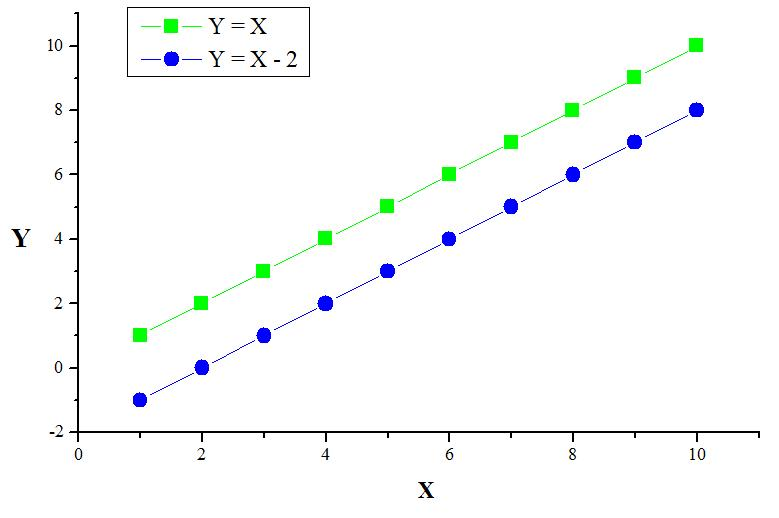
\includegraphics{examples/images/graph.jpg}
}

\caption{
\label{graph-fig}
     Линейные функции.}
\end {center}
\end {figure}
Ссылаемся на график ~\ref{graph-fig}.
Ссылка на статью: \cite{mbgd}

\specialsection{Выводы}
Жизнь --- тлен.
\pagebreak

\specialsection{Заключение}

% Библиография в cpsconf стиле
% Аргумент {1} ниже включает переопределенный стиль с выравниванием слева
\begin{thebibliography}{1}
\bibitem{mbgd} S. Ghadimi, G. Lan, and H. Zhang. \flqq Mini-batch stochastic approximation methods for nonconvex stochastic composite optimization\frqq. Mathematical Programming, 2016.

\bibitem{consensus_basics} R Olfati-Saber, JA Fax, RM Murray. \flqq Consensus and cooperation in networked multi-agent systems\frqq. IEEE, 2007.

\bibitem{consensus_basics_2} R. Olfati-Saber and R. M. Murray, \flqq Consensus problems in networks of agents with switching topology and time-delays\frqq. IEEE Transactions on Automatic Control, vol. 49, no. 9, pp. 1520-1533, Sept. 2004, doi: 10.1109/TAC.2004.834113.

\bibitem{fast_averaging} Boyd S, \flqq Convex optimization of graph Laplacian eigenvalues \frqq. Proceedings of the International Congress of Mathematicians. – 2006. – Т. 3. – №. 1-3. – С. 1311-1319.

\bibitem{decentralized_sgd} Koloskova A. et al. \flqq A unified theory of decentralized SGD with changing topology and local updates\frqq. International Conference on Machine Learning. – PMLR, 2020. – С. 5381-5393.

\bibitem{o1} O. Dekel, R. Gilad-Bachrach, O. Shamir, and L. Xiao. \flqq Optimal distributed online prediction using mini-batches\frqq. Journal of Machine Learning Research, 2012.

\bibitem{o2} A. Agarwal and J. C. Duchi. \flqq Distributed delayed stochastic optimization \frqq. In NIPS, 2011.

\bibitem{o3} H. R. Feyzmahdavian, A. Aytekin, and M. Johansson. \flqq An asynchronous mini-batch algorithm for regularized stochastic optimization\frqq. IEEE Transactions on Automatic Control, 2016.

\bibitem{o4} T. Paine, H. Jin, J. Yang, Z. Lin, and T. Huang. \flqq Gpu asynchronous stochastic gradient descent to speed up neural network training\frqq. arXiv preprint arXiv:1312.6186, 2013.

\bibitem{o5} B. Recht, C. Re, S. Wright, and F. Niu. Hogwild: \flqq A lock-free approach to parallelizing stochastic gradient descent\frqq. In Advances in neural information processing systems, 2011.

\bibitem{o6}  N. Luehr. \flqq Fast multi-gpu collectives with nccl\frqq. Nvidia blog, 2016.

\bibitem{o7}  P. Patarasuk and X. Yuan. \flqq Bandwidth optimal all-reduce algorithms for clusters of workstations\frqq. Journal of Parallel and Distributed Computing, 2009.

\bibitem{o8} Lian X. et al. \flqq Can decentralized algorithms outperform centralized algorithms? a case study for decentralized parallel stochastic gradient descent\frqq. arXiv preprint arXiv:1705.09056. – 2017.

\bibitem{o9} B. Sirb and X. Ye. \flqq Consensus optimization with delayed and stochastic gradients on decentralized networks\frqq. In Big Data, 2016.

\bibitem{o10} P. Bianchi, G. Fort, and W. Hachem. \flqq Performance of a distributed stochastic approximation algorithm\frqq. IEEE Transactions on Information Theory, 2013.

\bibitem{o11} Xiangru Lian, Wei Zhang, Ce Zhang, Ji Li. \flqq Asynchronous Decentralized Parallel Stochastic Gradient Descent\frqq. Proceedings of the 35th International Conference on Machine Learning, PMLR 80:3043-3052, 2018.

\end{thebibliography}
\end{document}